\section{Schieberegister}
\subsection{SRAM}
\begin{center}
    \begin{minipage}{0.45\linewidth}
        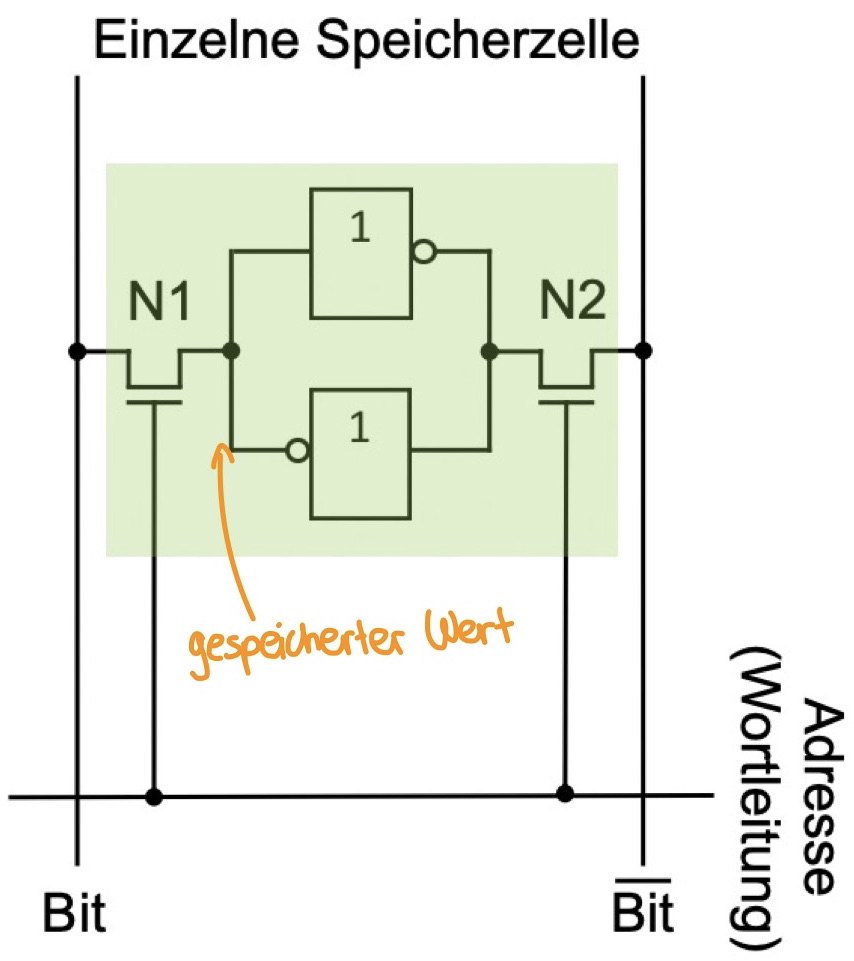
\includegraphics[width = 30mm]{images/sram_store.JPG}
    \end{minipage}
    \hfill
    \begin{minipage}{0.5\linewidth}
        \cemph[black]{Wortleitung}: Anwählen Speicherzelle\\
        \cemph[black]{Bitleitung}: Speicherinhalt lesen oder setzten
        \begin{center}
            \begin{tabular}{c c l}
                Bit & $\overline{\text{Bit}}$ & \\
                1 & 0 & 1 schreiben\\
                0 & 1 & 0 schreiben\\
                1 & 1 & lesen\\
                \multicolumn{3}{l}{Wortleitung bei allen 1.}
            \end{tabular}
        \end{center}
    \end{minipage}
\end{center}
\begin{itemize}
    \item Gespeicherte Wert steht immer auf linker Seite (Bit)
    \item Beim Lesen gibt Bit den Wert zurück; $\overline{\text{Bit}}$ den Invertierten.
    \item Beim Schreiben muss Bit auf den gewünschten Wert und $\overline{\text{Bit}}$ auf den Invertierten gesetzt werden.
\end{itemize}
\paragraph{Lesen}\mbox{}\\
\begin{center}
    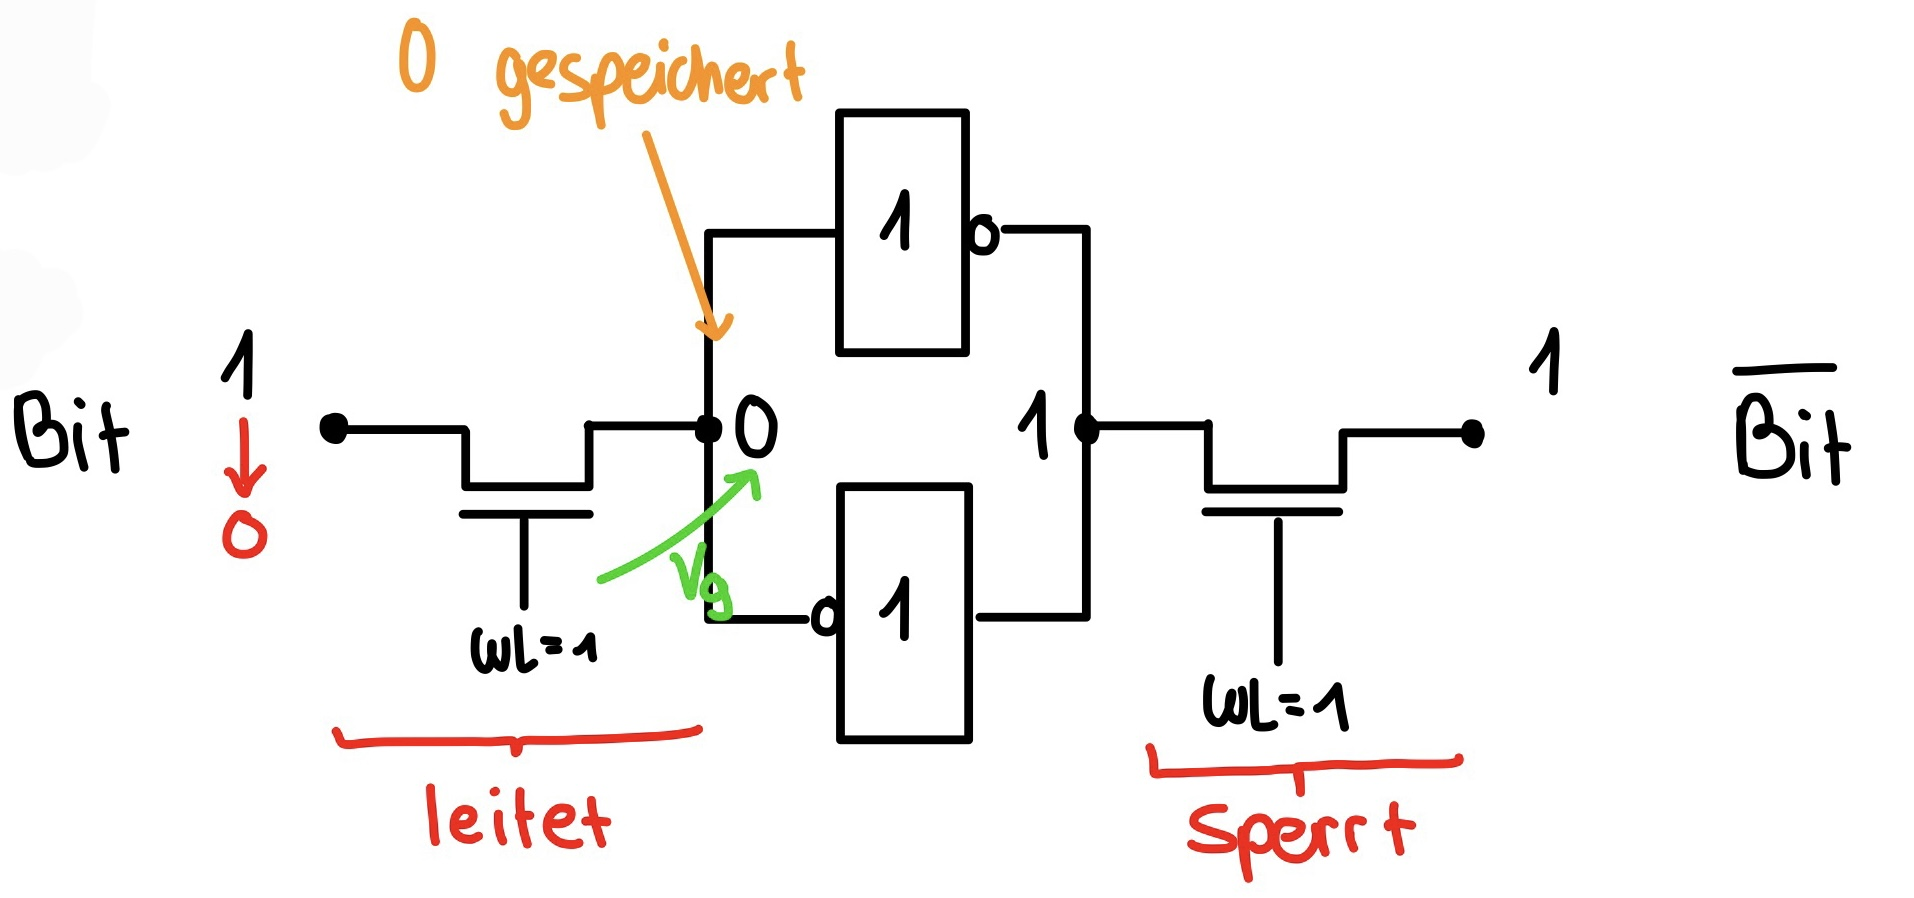
\includegraphics[width = 50mm]{images/sram_read.JPG}
\end{center}
\paragraph{1 Schreiben}\mbox{}\\
\begin{center}
    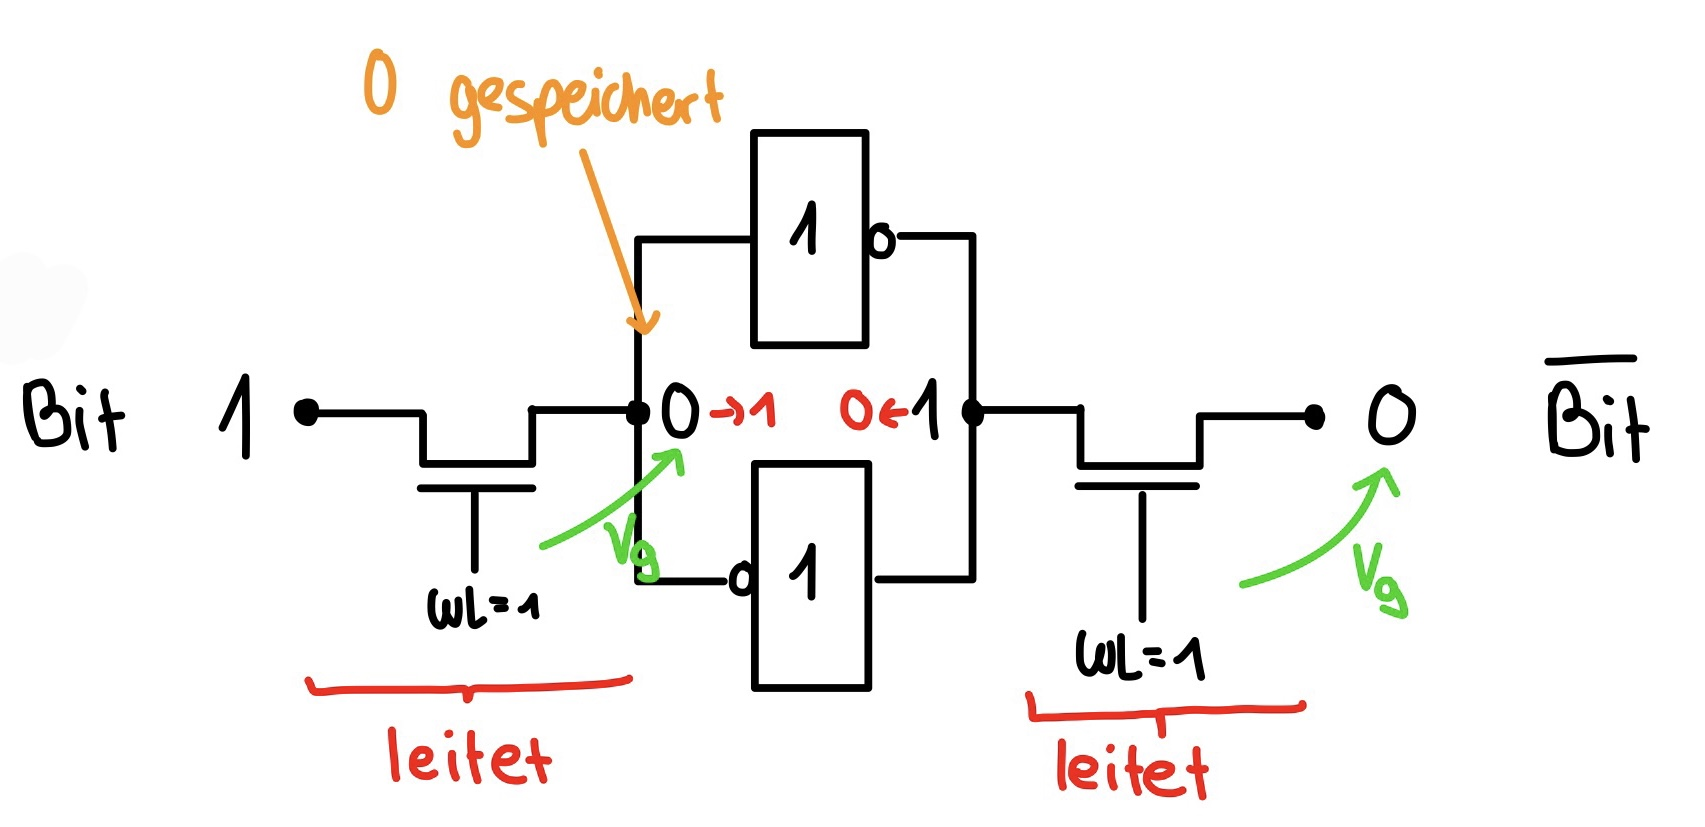
\includegraphics[width =50mm]{images/sram_write.JPG}
\end{center}
\paragraph{0 Schreiben} Gleich wie Schreiben einer 1, aber Bit = 0.

\subsection{DRAM}
\begin{center}
    \begin{minipage}{0.45\linewidth}
        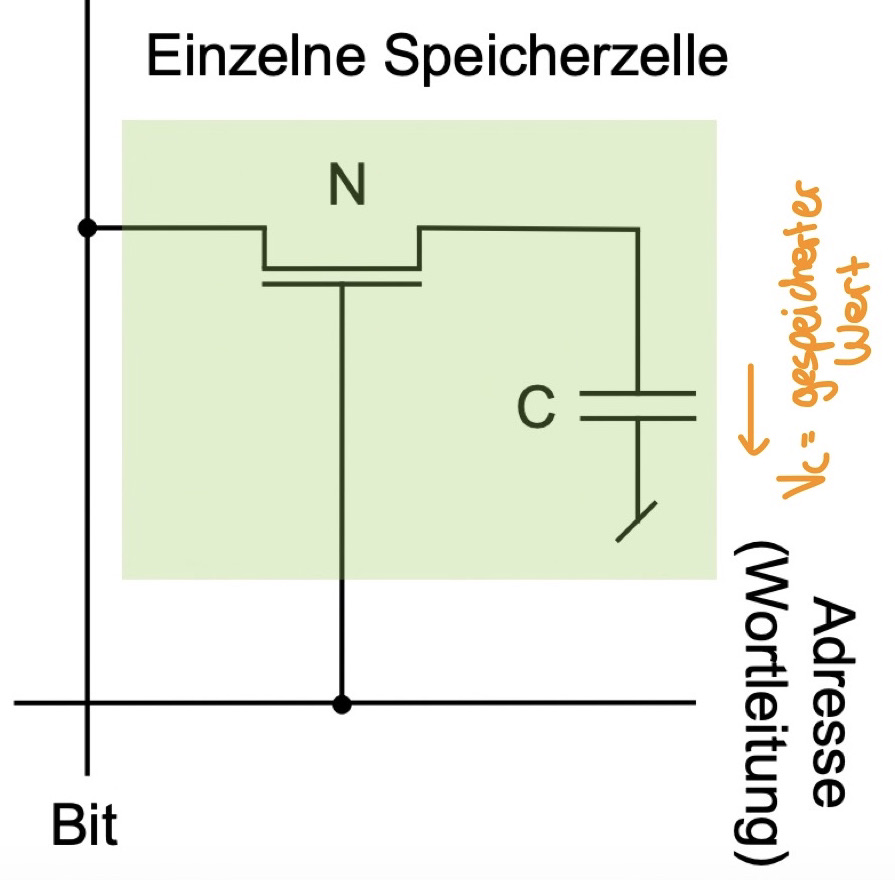
\includegraphics[width = 30mm]{images/dram_store.JPG}
    \end{minipage}
    \hfill
    \begin{minipage}{0.5\linewidth}
        \cemph[black]{Wortleitung}: Anwählen Speicherzelle\\
        \cemph[black]{Bitleitung}: Speicherinhalt lesen oder setzten\\
        \cemph[black]{Schreiben}: Bitleitung wird auf gewünschten Wert gesetzt $\rightarrow$ Kondensator: lädt, entlädt oder bleibt gleich.\\
        \cemph[black]{Lesen}: Parasitäre Kapazität wird ausgenutzt, um aus Veränderung von $V_{\text{out}}$ gespeicherten Wert zu ermitteln.
    \end{minipage}
\end{center}

\subsection{ROM}
Read-Only-Memory wird zur Herstellungszeit als 0 oder 1 programmiert.
\begin{center}
    \begin{minipage}{0.45\linewidth}
        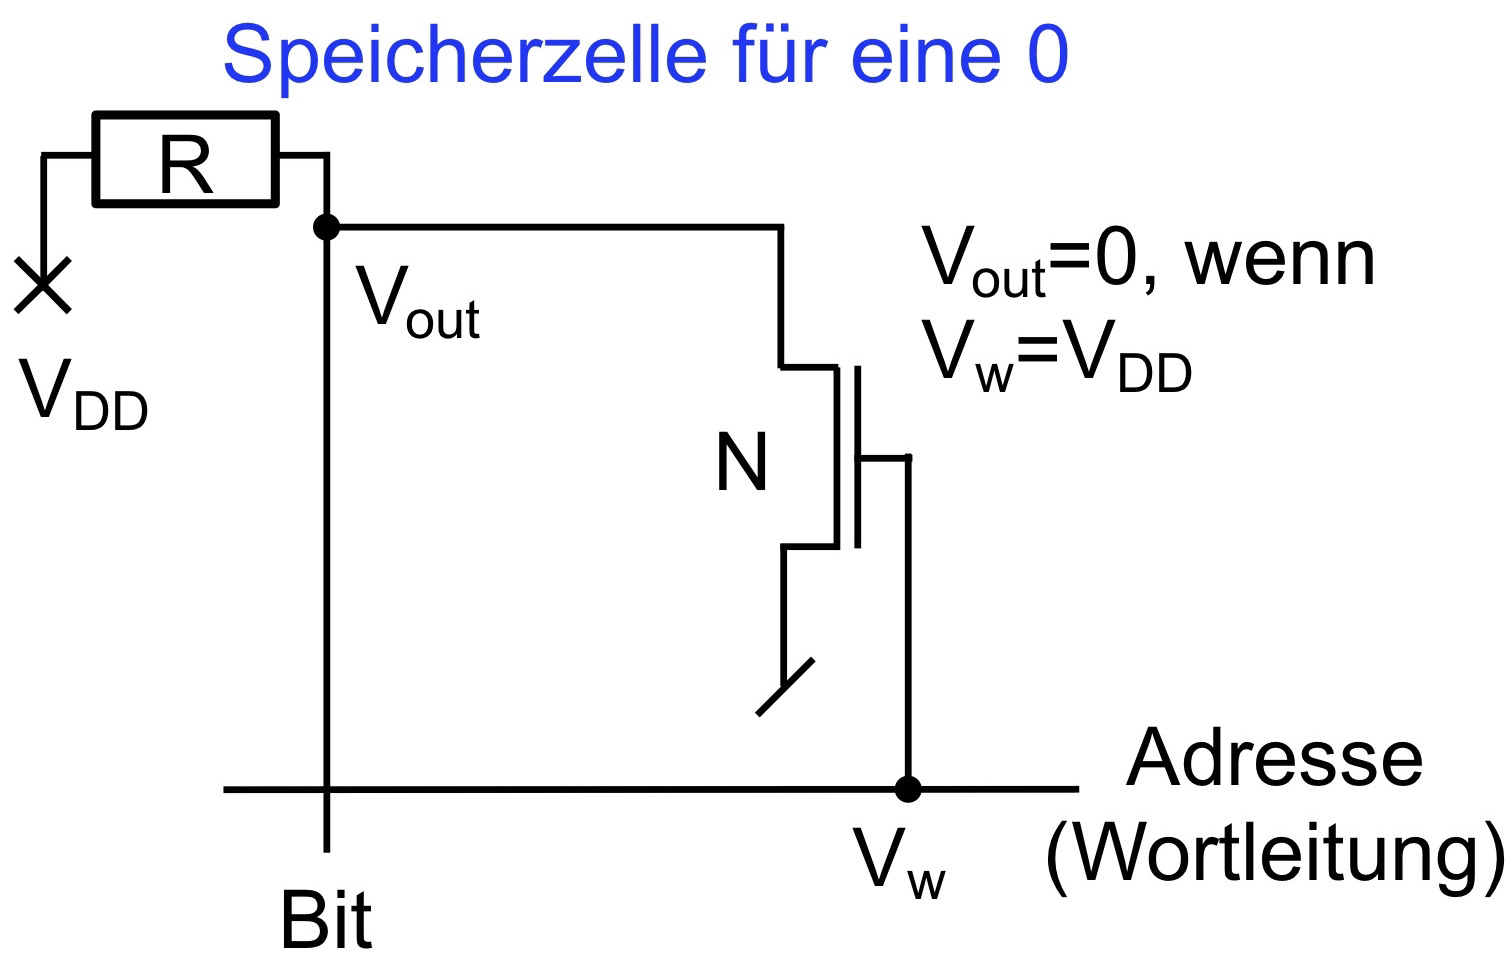
\includegraphics[width = 30mm]{images/rom_0.JPG}
    \end{minipage}
    \hfill
    \begin{minipage}{0.45\linewidth}
        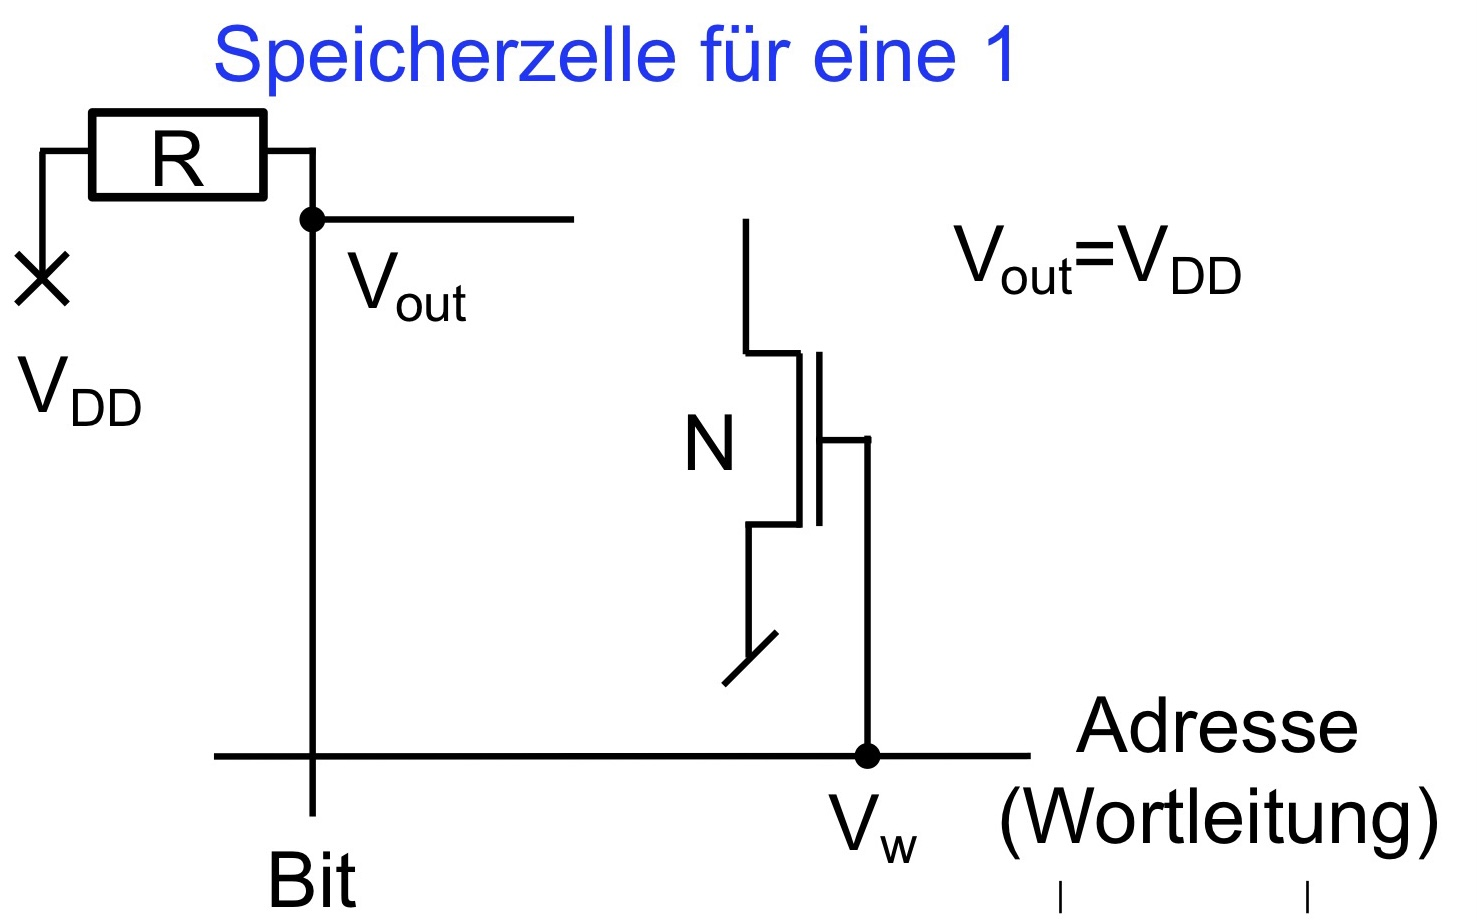
\includegraphics[width = 30mm]{images/rom_1.JPG}
    \end{minipage}
\end{center}